% ---------------------------------------------------------------------------------------
% MODELO DE TCC - INSTITUTO FEDERAL DE SERGIPE (IFS)
% ---------------------------------------------------------------------------------------
% Autor do Modelo: Mikael dos Santos Gois (mikaelgois1@gmail.com)
% Baseado nos modelos de: 
%   - Diogo D. Moreira (TCC, Dissertação e Tese)
%   - DECOM/UFOP (Monografia de Ciência da Computação)
% Modelo Base: abnTeX2 adaptado para as normativas internas de TCC do IFS (Art. 31 e 34)
% Versão: 1.0 (2026)
% ---------------------------------------------------------------------------------------
% Este arquivo faz parte de um modelo opensource para estudantes do IFS.
% Não remova os créditos dos autores originais e do modelo base.
% Este modelo é fornecido "no estado em que se encontra", sem garantias de qualquer tipo.
% ---------------------------------------------------------------------------------------

% -------------------------------------------------------------------
% 1. DEFINIÇÕES GERAIS (Normas IFS - Art. 34)
% -------------------------------------------------------------------
\documentclass[12pt, openright, oneside, a4paper, english, brazil]{abntex2}

% Variáveis adicionais
\providecommand{\imprimirautorcite}{}
\newcommand{\autorcite}[1]{\renewcommand{\imprimirautorcite}{#1}}
\providecommand{\imprimirorientadorcite}{}
\newcommand{\orientaddorcite}[1]{\renewcommand{\imprimirorientadorcite}{#1}}
\providecommand{\imprimircoorientadorcite}{}
\newcommand{\coorientaddorcite}[1]{\renewcommand{\imprimircoorientadorcite}{#1}}

% --- PACOTES BÁSICOS ---
\usepackage{times}              % Fonte Times New Roman
\usepackage[T1]{fontenc}        % Selecao de codigos de fonte.
\usepackage[utf8]{inputenc}     % Codificacao do arquivo (conversão automática dos acentos)
\usepackage{indentfirst}        % Indenta o primeiro parágrafo de cada seção.
\usepackage{color}              % Controle das cores
\usepackage{graphicx}           % Inclusão de gráficos
\usepackage{microtype}          % para melhorias de justificação
\usepackage[alf]{abntex2cite}   % Citações padrão ABNT

% --- CONFIGURAÇÕES DE MARGENS ---
% \setlmargin{3cm} \setrmargin{2cm} \settmargin{3cm} \setbmargin{2cm}
\usepackage[a4paper, top=3.0cm, bottom=2.0cm, left=3.0cm, right=2.0cm]{geometry}
\linespread{1.5}                % Espaçamento 1,5

% -------------------------------------------------------------------
% DADOS DO ALUNO E DO TRABALHO (PREENCHA AQUI)
% -------------------------------------------------------------------
\titulo{LUSO: Um Ecossistema Opensource para o Ensino Localizado de Programação}
\autor{Mikael dos Santos Gois} 
\autorcite{Gois, Mikael Gois}
\local{Itabaiana/SE}
\data{2026}
\orientador{Prof. Me. Marlos Tacio Silva}
\orientaddorcite{Silva, Marlos Tacio}
\coorientador{Prof. Dr. José Aprígio Carneiro Neto} % Deixe vazio se não houver
\coorientaddorcite{Neto, José Aprígio Carneiro} % Deixe vazio se não houver
\logoinstituicao{
\includegraphics[width=3cm]{figuras/logo-instituicao.png}} % Caminho da logo. Deixe vazio se não houver
\instituicao{
  \par
  INSTITUTO FEDERAL DE SERGIPE
  \par
  COORDENADORIA DO CURSO DE BACHAREL EM CIÊNCIA DA COMPUTAÇÃO
  \par
  CAMPUS ITABAIANA
  }
\tipotrabalho{Trabalho de Conclusão de Curso (Bacharelado)}
\preambulo{Monografia apresentada à Coordenação de Ciência da Computação do Campus Itabaiana, do Instituto Federal de Sergipe (IFS), como pré-requisito para obtenção do grau de Bacharel em Ciência da Computação.}

% --- CONFIGURAÇÕES DE PDF ---
\makeatletter
\hypersetup{
    pdftitle={\@title}, 
    pdfauthor={\@author},
    pdfsubject={\imprimirpreambulo},
    colorlinks=false,   % links coloridos? (mantenha false para impressão)
}
\makeatother

% -------------------------------------------------------------------
% INÍCIO DO DOCUMENTO
% -------------------------------------------------------------------
\begin{document}

\frenchspacing

% --- ELEMENTOS PRÉ-TEXTUAIS ---
\imprimircapa
\imprimirfolhaderosto

% ---------------------------------------------------------------------------------------
% MODELO DE TCC - INSTITUTO FEDERAL DE SERGIPE (IFS)
% ---------------------------------------------------------------------------------------
% Autor do Modelo: Mikael dos Santos Gois (mikaelgois1@gmail.com)
% Baseado nos modelos de: 
%   - Diogo D. Moreira (TCC, Dissertação e Tese)
%   - DECOM/UFOP (Monografia de Ciência da Computação)
% Modelo Base: abnTeX2 adaptado para as normativas internas de TCC do IFS (Art. 31 e 34)
% Versão: 1.0 (2026)
% ---------------------------------------------------------------------------------------
% Este arquivo faz parte de um modelo opensource para estudantes do IFS.
% Não remova os créditos dos autores originais e do modelo base.
% Este modelo é fornecido "no estado em que se encontra", sem garantias de qualquer tipo.
% ---------------------------------------------------------------------------------------

% Modelo de ficha catalográfica. Você deverá substituir esta
% folha na versão final da monografia por um pdf fornecido pela biblioteca.
% Salve o modelo oficial como ficha_catalografica.pdf na raiz do projeto,
% e use o comando abaixo para inseri-lo na versão final do texto.

%\begin{fichacatalografica}
%    \includepdf{ficha_catalografica.pdf}
%\end{fichacatalografica}

%% Modelo de Como fazer a Folha/Ficha Catalográfica:

\begin{fichacatalografica}
  \sffamily
  \vspace*{\fill}					% Posição vertical
  \begin{center}					% Minipage Centralizado
    \fbox{
      \begin{minipage}[c][8cm]{14cm}		% Largura
        \small
        \begin{center}
          {Isto é apenas um exemplo e deve ser substituído pela ficha catalográfica oficial fornecida pela biblioteca do IFS.}
        \end{center}
        \imprimirautorcite.
        %Sobrenome, Nome do autor

        \hspace{0.5cm}  \\
        \imprimirtitulo. / \imprimirautor. -- \imprimirlocal, \imprimirano.

        % \hspace{0.5cm} \pageref{LastPage} p. 1 :il. (colors; grafs; tabs).\\

        \hspace{0.5cm}  \\
        {Trabalho de conclusão de curso (Bacharelado em Ciência da
        Computação) – Instituto Federal de Educação, Ciência e Tecnologia de
        Sergipe – IFS, \imprimirano. \\}

        \hspace{0.5cm} \imprimirorientadorRotulo~\imprimirorientador.
        \ifthenelse{\equal{\imprimircoorientador}{}}{}{ \imprimircoorientadorRotulo~\imprimircoorientador \\}

        % \hspace{0.5cm}
        % \parbox[t]{\textwidth}{\imprimirtipotrabalho~--~\imprimirinstituicao, ~ \\
        %   \imprimirinstituto, ~\imprimirdepartamento,~\imprimirano.}\\

        \hspace{0.5cm} % Palavras-chave do trabalho
        1. Palavra-chave.
        2. Palavra-chave.
        2. Palavra-chave.
        3. Palavra-chave.
        4. Palavra-chave.
        5. Palavra-chave.
        I. IFS.
        II. \imprimirautorcite.
        III. \imprimirorientadorcite.
        \ifthenelse{\equal{\imprimircoorientadorcite}{}}{IV. \imprimirtitulo.}{IV. \imprimircoorientadorcite. V. \imprimirtitulo.}
      \end{minipage}
    }
  \end{center}
\end{fichacatalografica}
\addtocounter{page}{-1} % Subtrai 1 da contagem total de páginas

% ---------------------------------------------------------------------------------------
% MODELO DE TCC - INSTITUTO FEDERAL DE SERGIPE (IFS)
% ---------------------------------------------------------------------------------------
% Autor do Modelo: Mikael dos Santos Gois (mikaelgois1@gmail.com)
% Baseado nos modelos de: 
%   - Diogo D. Moreira (TCC, Dissertação e Tese)
%   - DECOM/UFOP (Monografia de Ciência da Computação)
% Modelo Base: abnTeX2 adaptado para as normativas internas de TCC do IFS (Art. 31 e 34)
% Versão: 1.0 (2026)
% ---------------------------------------------------------------------------------------
% Este arquivo faz parte de um modelo opensource para estudantes do IFS.
% Não remova os créditos dos autores originais e do modelo base.
% Este modelo é fornecido "no estado em que se encontra", sem garantias de qualquer tipo.
% ---------------------------------------------------------------------------------------

\begin{folhadeaprovacao}

  \begin{center}
    {\ABNTEXchapterfont\large\imprimirautor}

    \vspace{2cm}
    \begin{center}
      \ABNTEXchapterfont\bfseries\large\imprimirtitulo
    \end{center}

  \end{center}

  \vspace{1cm}
  \begin{flushright} \parbox{0.6\linewidth}
    \imprimirpreambulo
  \end{flushright}

  \vspace{1cm}
  \begin{center}
    Trabalho defendido e aprovado em: 01/01/2026 % Preencha a data}
  \end{center}

  \begin{center}
    \textbf{BANCA EXAMINADORA}

    \vfill
    \rule{10cm}{.1pt} \\ {\imprimirorientador \space(Orientador) \\ Instituto Federal de Sergipe}

    \ifthenelse{\equal{\imprimircoorientador}{}}{}{
    \vfill
    \rule{10cm}{.1pt} \\ {\imprimircoorientador \space(Coorientador) \\ Instituto Federal de Sergipe}
    }

    \vfill
    \rule{10cm}{.1pt} \\ {Prof. Nome do Membro 1 (Membro examinador) \\ Instituto Federal de Sergipe}

    \vfill
    \rule{10cm}{.1pt} \\ {Prof. Nome do Membro 2 (Membro examinador) \\ Instituto Federal de Sergipe}

  \end{center}

\end{folhadeaprovacao}
% ---------------------------------------------------------------------------------------
% MODELO DE TCC - INSTITUTO FEDERAL DE SERGIPE (IFS)
% ---------------------------------------------------------------------------------------
% Autor do Modelo: Mikael dos Santos Gois (mikaelgois1@gmail.com)
% Baseado nos modelos de: 
%   - Diogo D. Moreira (TCC, Dissertação e Tese)
%   - DECOM/UFOP (Monografia de Ciência da Computação)
% Modelo Base: abnTeX2 adaptado para as normativas internas de TCC do IFS (Art. 31 e 34)
% Versão: 1.0 (2026)
% ---------------------------------------------------------------------------------------
% Este arquivo faz parte de um modelo opensource para estudantes do IFS.
% Não remova os créditos dos autores originais e do modelo base.
% Este modelo é fornecido "no estado em que se encontra", sem garantias de qualquer tipo.
% ---------------------------------------------------------------------------------------

\begin{dedicatoria}
  \vspace*{\fill}
  \noindent
  \begin{flushright}
    \begin{em}
      \begin{minipage}{.5\textwidth}
        \begin{OnehalfSpacing}
          \textit{Espaço para prestar uma homenagem ou dedicar o trabalho a alguém. Não necessariamente
            pessoas envolvidas com o seu trabalho, mas que tenham sido importantes para a sua trajetória
            acadêmica ou pessoal.}
        \end{OnehalfSpacing}
      \end{minipage}
    \end{em}
  \end{flushright}
\end{dedicatoria}
% =======================================================================================
% MODELO DE TCC - INSTITUTO FEDERAL DE SERGIPE (IFS)
% =======================================================================================
% Autores do Modelo (discentes de Ciência da Computação - IFS, Campus Itabaiana):
%   Mikael dos Santos Gois
%   Talyson Rodrigues Silva Nascimento
%   Kauan Gutierrez Santos Estácio
% Modelo Base: abnTeX2, adaptado para as normativas internas de TCC do IFS (Art. 31 e 34)
% Créditos dos modelos base (abnTeX2, DECOM/UFOP e Diogo D. Moreira) e das imagens: ver NOTICE
% Licença: CC BY-SA 4.0 (ver LICENSE)
% Este arquivo faz parte de um modelo opensource para estudantes do IFS.
% Não remova os créditos dos autores originais e do modelo base.
% Este modelo é fornecido "no estado em que se encontra", sem garantias de qualquer tipo.
% =======================================================================================

\begin{agradecimentos}
  % Não deve haver indentação.
  \noindent Espaço para agradecer às pessoas e/ou instituições que contribuíram de forma relevante à elaboração do trabalho.
\end{agradecimentos}
% ---------------------------------------------------------------------------------------
% MODELO DE TCC - INSTITUTO FEDERAL DE SERGIPE (IFS)
% ---------------------------------------------------------------------------------------
% Autor do Modelo: Mikael dos Santos Gois (mikaelgois1@gmail.com)
% Atualizado por: Talyson Rodrigues Silva Nascimento (talyson.rodigues@gmail.com)
% Baseado nos modelos de: 
%   - Diogo D. Moreira (TCC, Dissertação e Tese)
%   - DECOM/UFOP (Monografia de Ciência da Computação)
% Modelo Base: abnTeX2 adaptado para as normativas internas de TCC do IFS (Art. 31 e 34)
% Versão: 1.0 (2026)
% ---------------------------------------------------------------------------------------
% Este arquivo faz parte de um modelo opensource para estudantes do IFS.
% Não remova os créditos dos autores originais e do modelo base.
% Este modelo é fornecido "no estado em que se encontra", sem garantias de qualquer tipo.
% --------------------------------------------------------------
\thispagestyle{empty} % Contada, mas não numerada

\vspace*{\fill} %Posicionada na parte inferior 

\begin{flushright}
    \begin{minipage}{.5\textwidth} % Do meio da mancha à margem direita 
        \begin{OnehalfSpacing} % Espaçamento 1,5 — NBR 14724:2024, 5.2 não excepciona a epígrafe
            \textit{“Alguma citação importante para a construção do trabalho. A fonte deve ser indicada e também deve constar na lista de referências bibliográficas.”}
            
            \vspace{1em}
            (Nome do Autor) % Indicação de autoria
        \end{OnehalfSpacing}
    \end{minipage}
\end{flushright}
% ---------------------------------------------------------------------------------------
% MODELO DE TCC - INSTITUTO FEDERAL DE SERGIPE (IFS)
% ---------------------------------------------------------------------------------------
% Autor do Modelo: Mikael dos Santos Gois (mikaelgois1@gmail.com)
% Baseado nos modelos de: 
%   - Diogo D. Moreira (TCC, Dissertação e Tese)
%   - DECOM/UFOP (Monografia de Ciência da Computação)
% Modelo Base: abnTeX2 adaptado para as normativas internas de TCC do IFS (Art. 31 e 34)
% Versão: 1.0 (2026)
% ---------------------------------------------------------------------------------------
% Este arquivo faz parte de um modelo opensource para estudantes do IFS.
% Não remova os créditos dos autores originais e do modelo base.
% Este modelo é fornecido "no estado em que se encontra", sem garantias de qualquer tipo.
% ---------------------------------------------------------------------------------------

\begin{resumo}
  A programação é uma competência fundamental no século XXI, mas o ensino introdutório enfrenta barreiras
  significativas que desmotivam o aprendizado inicial, como a barreira da língua inglesa e a complexidade
  sintática prematura. Este trabalho apresenta o projeto Luso, uma linguagem de programação educacional
  projetada com sintaxe em português. Baseado nas teorias de Localização de Software e Programação Gradual,
  o Luso visa reduzir a carga cognitiva de estudantes novatos, servindo como um andaime (scaffolding)
  para a transição futura para linguagens profissionais como Java e Python. O projeto propõe um ecossistema
  que inclui um transpilador, uma IDE e suporte a ferramentas de desenvolvimento terceiras, buscando
  alinhar a tecnologia à didática do professor. Além disso, o projeto conta com documentação educacional
  para usuários e documentação técnica para contribuidores do projeto.

  \vspace{\onelineskip}

  \noindent
  \textbf{Palavras-chave}: Ensino de Programação; Linguagens Graduais; Localização de Software; Barreira
  de Sintaxe; Carga Cognitiva.
\end{resumo}
% ---------------------------------------------------------------------------------------
% MODELO DE TCC - INSTITUTO FEDERAL DE SERGIPE (IFS)
% ---------------------------------------------------------------------------------------
% Autor do Modelo: Mikael dos Santos Gois (mikaelgois1@gmail.com)
% Baseado nos modelos de: 
%   - Diogo D. Moreira (TCC, Dissertação e Tese)
%   - DECOM/UFOP (Monografia de Ciência da Computação)
% Modelo Base: abnTeX2 adaptado para as normativas internas de TCC do IFS (Art. 31 e 34)
% Versão: 1.0 (2026)
% ---------------------------------------------------------------------------------------
% Este arquivo faz parte de um modelo opensource para estudantes do IFS.
% Não remova os créditos dos autores originais e do modelo base.
% Este modelo é fornecido "no estado em que se encontra", sem garantias de qualquer tipo.
% ---------------------------------------------------------------------------------------

\begin{resumo}[Abstract]
  \begin{otherlanguage*}{english}
    Programming is a fundamental skill in the 21st century, but introductory teaching faces significant
    barriers that discourage initial learning, such as the English language barrier and premature syntactic
    complexity. This work presents the Luso project, an educational programming language designed with
    syntax in Portuguese. Based on the theories of Software Localization and Gradual Programming, Luso
    aims to reduce the cognitive load of novice students, serving as a scaffolding for the future transition
    to professional languages such as Java and Python. The project proposes an ecosystem that includes
    a transpiler, an IDE, and support for third-party development tools, seeking to align technology
    with the teacher's teaching methods. In addition, the project has educational documentation for users
    and technical documentation for project contributors.

    \vspace{\onelineskip}

    \noindent
    \textbf{Keywords}: Teaching Programming; Gradual Languages; Software Localization; Syntax Barrier; Cognitive Load.
  \end{otherlanguage*}
\end{resumo}
% ---------------------------------------------------------------------------------------
% MODELO DE TCC - INSTITUTO FEDERAL DE SERGIPE (IFS)
% ---------------------------------------------------------------------------------------
% Autor do Modelo: Mikael dos Santos Gois (mikaelgois1@gmail.com)
% Baseado nos modelos de: 
%   - Diogo D. Moreira (TCC, Dissertação e Tese)
%   - DECOM/UFOP (Monografia de Ciência da Computação)
% Modelo Base: abnTeX2 adaptado para as normativas internas de TCC do IFS (Art. 31 e 34)
% Versão: 1.0 (2026)
% ---------------------------------------------------------------------------------------
% Este arquivo faz parte de um modelo opensource para estudantes do IFS.
% Não remova os créditos dos autores originais e do modelo base.
% Este modelo é fornecido "no estado em que se encontra", sem garantias de qualquer tipo.
% ---------------------------------------------------------------------------------------

% --- Ficha Catalográfica (Geralmente fornecida pela biblioteca) ---
% \include{01-pre-textuais/ficha-catalografica}

% --- Dedicatória, Agradecimentos e Epígrafe ---
\include{01-pre-textuais/dedicatoria}
\include{01-pre-textuais/agradecimentos}
\include{01-pre-textuais/epigrafe}

% --- Resumos ---
\include{01-pre-textuais/resumo}
\include{01-pre-textuais/abstract}

% --- Listas ---
\pdfbookmark[0]{\listfigurename}{lof}
\listoffigures*
\cleardoublepage
\listoftables*
\cleardoublepage
\pdfbookmark[0]{\contentsname}{toc}
\tableofcontents*
\cleardoublepage

% --- ELEMENTOS TEXTUAIS ---
\textual
% ---------------------------------------------------------------------------------------
% MODELO DE TCC - INSTITUTO FEDERAL DE SERGIPE (IFS)
% ---------------------------------------------------------------------------------------
% Autor do Modelo: Mikael dos Santos Gois (mikaelgois1@gmail.com)
% Baseado nos modelos de: 
%   - Diogo D. Moreira (TCC, Dissertação e Tese)
%   - DECOM/UFOP (Monografia de Ciência da Computação)
% Modelo Base: abnTeX2 adaptado para as normativas internas de TCC do IFS (Art. 31 e 34)
% Versão: 1.0 (2026)
% ---------------------------------------------------------------------------------------
% Este arquivo faz parte de um modelo opensource para estudantes do IFS.
% Não remova os créditos dos autores originais e do modelo base.
% Este modelo é fornecido "no estado em que se encontra", sem garantias de qualquer tipo.
% ---------------------------------------------------------------------------------------

% [O que aparece no PDF Bookmark] {O que aparece impresso no documento}
\chapter[Introdução]{INTRODUÇÃO} \label{sec:introducao}
A introdução é a seção inicial do trabalho, onde o tema é apresentado e contextualizado.
Nela, o autor deve expor a motivação para a escolha do tema, os objetivos do estudo, a justificativa da relevância do trabalho e a metodologia adotada para alcançar os resultados esperados.
A introdução deve ser clara e objetiva, fornecendo ao leitor uma visão geral do que será abordado no restante do trabalho.
\cite{kitchenham2007guidelinesOnline}

\cite[text]{kitchenham2007guidelines}
% =======================================================================================
% MODELO DE TCC - INSTITUTO FEDERAL DE SERGIPE (IFS)
% =======================================================================================
% Autores do Modelo (discentes de Ciência da Computação - IFS, Campus Itabaiana):
%   Mikael dos Santos Gois
%   Talyson Rodrigues Silva Nascimento
%   Kauan Gutierrez Santos Estácio
% Modelo Base: abnTeX2, adaptado para as normativas internas de TCC do IFS (Art. 31 e 34)
% Créditos dos modelos base (abnTeX2, DECOM/UFOP e Diogo D. Moreira) e das imagens: ver NOTICE
% Licença: CC BY-SA 4.0 (ver LICENSE)
% Este arquivo faz parte de um modelo opensource para estudantes do IFS.
% Não remova os créditos dos autores originais e do modelo base.
% Este modelo é fornecido "no estado em que se encontra", sem garantias de qualquer tipo.
% =======================================================================================

% [O que aparece no PDF Bookmark] {O que aparece impresso no documento}
\chapter[Fundamentação Teórica]{FUNDAMENTAÇÃO TEÓRICA}
\label{sec:fundamentacao-teorica}

% 1. TEXTO DE ABERTURA 
A fundamentação teórica é a seção inicial de desenvolvimento do trabalho, onde os conceitos principais são apresentados e contextualizados. Nela, o autor deve expor a revisão da literatura e detalhar as tecnologias escolhidas, criando a base de conhecimento necessária para que o leitor compreenda a viabilidade do estudo. Esta seção deve ser clara, objetiva e devidamente embasada em autores reconhecidos pela comunidade científica.

Neste capítulo, serão abordados os conceitos fundamentais sobre [INSERIR TEMA 1], as características da ferramenta [INSERIR TEMA 2] e o funcionamento do [INSERIR TEMA 3].
% EXEMPLO DE SEÇÃO COM INSERÇÃO DE FIGURA 
% ------------------------------------------------------------------------------
\section{Estrutura e Arquitetura de Sistemas}

% DICA PARA O ESTUDANTE:
% Sempre referencie a figura no texto ANTES dela aparecer, usando o comando \ref{}.
Para compreender o funcionamento da solução proposta, é essencial analisar os modelos clássicos de processamento. A arquitetura computacional padrão pode ser visualizada na Figura \ref{fig:exemplo_arquitetura}. Nela estão representados todos os componentes principais de interação.

% BLOCO PADRÃO PARA INSERIR FIGURAS (ESTILO ABNT / IFS)
% Substitua o título, o caminho da imagem e a fonte pelos dados do seu TCC.
\begin{figure}[htb]
    \centering
    \caption{Título da sua ilustração (Ex: Arquitetura de Von Neumann)}
    % Ajuste a largura (width) conforme necessário e coloque o nome do seu arquivo
    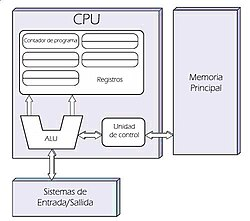
\includegraphics[width=0.7\textwidth]{figuras/Arquitecturaneumann.jpg}
    % DICA: a fonte vai logo abaixo da ilustração, com a expressão de autoria
    % (NBR 14724:2024, 5.8). Se você criou a imagem:
    %   \fonte{Elaborada pelo autor (2026).}
    % Se adaptou de outro autor: \fonte{Adaptada de \citeonline{referencia}.}
    % A imagem de EXEMPLO deste modelo é o diagrama de von Neumann de David strigoi
    % (Wikimedia Commons, domínio público) - ver NOTICE. Substitua a imagem, o
    % arquivo em figuras/ e este crédito pelos seus.
    \fonte{Imagem de exemplo: David strigoi, Wikimedia Commons (domínio público). Adaptada de \citeonline{tanenbaum2013}.}
    \label{fig:exemplo_arquitetura}
\end{figure}

Como apresentado no fluxo da imagem anterior, [AQUI O ESTUDANTE DEVE EXPLICAR COM SUAS PALAVRAS O QUE A IMAGEM SIGNIFICA E COMO ELA SE APLICA AO SEU CONTEXTO].

%Ex Subseções
\subsection{O Paradigma do Processamento em PCs}

Exemplo de subseção, ou seção secundária.

%Ex: Subsubseções
\subsubsection{Limitações da Abordagem Baseada em PC}

Exemplo de seção terciária.
% =======================================================================================
% MODELO DE TCC - INSTITUTO FEDERAL DE SERGIPE (IFS)
% =======================================================================================
% Autores do Modelo (discentes de Ciência da Computação - IFS, Campus Itabaiana):
%   Mikael dos Santos Gois
%   Talyson Rodrigues Silva Nascimento
%   Kauan Gutierrez Santos Estácio
% Modelo Base: abnTeX2, adaptado para as normativas internas de TCC do IFS (Art. 31 e 34)
% Créditos dos modelos base (abnTeX2, DECOM/UFOP e Diogo D. Moreira) e das imagens: ver NOTICE
% Licença: CC BY-SA 4.0 (ver LICENSE)
% Este arquivo faz parte de um modelo opensource para estudantes do IFS.
% Não remova os créditos dos autores originais e do modelo base.
% Este modelo é fornecido "no estado em que se encontra", sem garantias de qualquer tipo.
% =======================================================================================

% [O que aparece no PDF Bookmark] {O que aparece impresso no documento}
\chapter[Trabalhos Correlatos]{TRABALHOS CORRELATOS} \label{sec:trabalhos-correlatos}

A análise de trabalhos correlatos permite mapear o estado da arte e identificar as abordagens metodológicas adotadas por outros pesquisadores para resolver problemas semelhantes. Nesta seção, são discutidas publicações recentes relacionadas à execução de algoritmos de inferência e coleta de dados inerciais.

Ao longo da literatura, nota-se que grande parte das implementações prioriza a execução de modelos computacionais em plataformas de alto desempenho. O Quadro \ref{qua:comparativo_trabalhos} sintetiza as principais diferenças de arquitetura e hardware entre os trabalhos analisados e a solução proposta nesta pesquisa.

% ---------------------------------------------------------------------------------------
% EXEMPLO DE QUADRO (DADOS TEXTUAIS) - NBR 14724:2024, 4.2.1.9 e 5.8
% ---------------------------------------------------------------------------------------
% DICA: dados TEXTUAIS (comparações, características, definições) vão em QUADRO. A norma
% trata o quadro como ILUSTRAÇÃO: identificação com palavra designativa + número +
% travessão + título, fonte logo abaixo e entrada na LISTA DE QUADROS (elemento próprio).
% No quadro, a moldura fechada é permitida.
% DICA: cite o quadro no texto ANTES dele aparecer (com \ref{}) e substitua o conteúdo
% de exemplo pelo seu.
\begin{quadro}[htb]
    \centering
    \caption{Comparativo entre os trabalhos correlatos e a solução proposta}
    \vspace{0.2cm}
    
    % DICA PARA O ESTUDANTE:
    % 'l' = alinhado à esquerda (ideal para colunas curtas, como o nome do Autor)
    % 'c' = centralizado (ideal para colunas com respostas curtas, como Sim/Não)
    % 'X' = coluna dinâmica que quebra o texto automaticamente e preenche o espaço da página
    \begin{tabularx}{\textwidth}{|l | X | X | X|}
        \hline
        \textbf{Autor (Ano)} & \textbf{[Inserir Critério 1]} & \textbf{[Inserir Critério 2]} & \textbf{[Inserir Critério 3]} \\
        \hline
        Sobrenome \emph{et al.} (2023) & Método longo que agora vai quebrar a linha sozinho & Baixo & Não \\
        \hline
        Sobrenome e Silva (2024)& Método Y & Médio & Sim \\
        \hline
        Sobrenome (2025)        & Método Z & Alto  & Não \\
        \hline
        \textbf{Proposta Atual} & \textbf{Método Inovador} & \textbf{Baixo} & \textbf{Sim} \\
        \hline
    \end{tabularx}
    
    \fonte{Elaborada pelo autor (2026).}
    \label{qua:comparativo_trabalhos}
\end{quadro}

Conforme evidenciado no Quadro \ref{qua:comparativo_trabalhos}, a principal distinção da proposta atual reside no.... Enquanto os trabalhos de Sobrenome \emph{et al.} (2023) e Sobrenome e Silva (2024) apresentam limitações quanto a [Citar o problema deles], a presente abordagem inova ao utilizar [Sua solução]. Essa escolha garante [Citar vantagem], preenchendo a lacuna identificada na literatura analisada.

% ---------------------------------------------------------------------------------------
% EXEMPLO DE TABELA (DADOS NUMÉRICOS) - NBR 14724:2024, 5.9 + Normas do IBGE
% ---------------------------------------------------------------------------------------
% DICA: dados NUMÉRICOS vão em TABELA, padronizada pelas Normas de apresentação tabular
% do IBGE (a NBR 14724:2024, 5.9, remete a elas):
%   - a moldura NÃO deve ter traços verticais que delimitem a tabela à esquerda e à
%     direita (IBGE, 4.3.3) - por isso o tabular abaixo não usa "|" nas laterais;
%   - no MÍNIMO três traços horizontais: topo, cabeçalho e rodapé (IBGE, 4.3.1);
%   - traços verticais apenas para DESTACAR parte do cabeçalho ou dos dados (IBGE, 4.3.2);
%   - a unidade de medida deve ser indicada no cabeçalho da coluna (IBGE, 4.6);
%   - recomenda-se alinhar os dados numéricos à direita (boa prática de leitura; a
%     norma do IBGE não fixa o alinhamento).
% DICA: se a tabela não couber em uma página, repita o cabeçalho e indique "continua"
% (primeira página), "continuação" (intermediárias) e "conclusão" (última), deixando o
% rodapé apenas na página de conclusão (IBGE).
% DICA: a tabela entra na LISTA DE TABELAS e é citada no texto com \ref{}.
A Tabela \ref{tab:selecao_rsl} exemplifica um dado numérico: a quantidade de trabalhos recuperados e selecionados em cada base de dados consultada.

\begin{table}[htb]
    \centering
    \caption{Trabalhos recuperados e selecionados por base de dados}
    \label{tab:selecao_rsl}
    \begin{tabular}{lrrr}
        \hline
        \textbf{Base de dados} & \textbf{Recuperados} & \textbf{Selecionados} & \textbf{Aproveitamento (\%)} \\
        \hline
        ACM Digital Library & 412 & 38 & 9,2 \\
        IEEE Xplore         & 356 & 41 & 11,5 \\
        Scopus              & 289 & 27 & 9,3 \\
        \textbf{Total}      & \textbf{1\,057} & \textbf{106} & \textbf{10,0} \\
        \hline
    \end{tabular}
    \fonte{Elaborada pelo autor (2026).}
\end{table}

Os números da Tabela \ref{tab:selecao_rsl} mostram que [explique, com suas palavras, o que os dados indicam: quantos trabalhos foram recuperados, quantos passaram pelos critérios de seleção e o que o percentual de aproveitamento revela sobre a busca].

% DICA PARA O ESTUDANTE:
% Sempre comente os resultados da tabela (ou do quadro) no parágrafo imediatamente
% abaixo, explicando com suas palavras o que os dados mostram.
%
% DICA: a expressão latina "et al." é grafada EM ITÁLICO no texto, nas citações
% e nas referências - assim como a própria ABNT a grafia nos exemplos da
% NBR 10520:2023 (6.1.2) e da NBR 6023:2025 (8.1.1.2). Use \emph{et al.}
% em textos escritos à mão; nas citações automáticas (\cite) e nas
% referências o próprio modelo já gera o itálico (entrada @abnt-options
% "opcoes-abnt" em referencias.bib + \citeoption{opcoes-abnt} em main.tex).
% =======================================================================================
% MODELO DE TCC - INSTITUTO FEDERAL DE SERGIPE (IFS)
% =======================================================================================
% Autores do Modelo (discentes de Ciência da Computação - IFS, Campus Itabaiana):
%   Mikael dos Santos Gois
%   Talyson Rodrigues Silva Nascimento
%   Kauan Gutierrez Santos Estácio
% Modelo Base: abnTeX2, adaptado para as normativas internas de TCC do IFS (Art. 31 e 34)
% Créditos dos modelos base (abnTeX2, DECOM/UFOP e Diogo D. Moreira) e das imagens: ver NOTICE
% Licença: CC BY-SA 4.0 (ver LICENSE)
% Este arquivo faz parte de um modelo opensource para estudantes do IFS.
% Não remova os créditos dos autores originais e do modelo base.
% Este modelo é fornecido "no estado em que se encontra", sem garantias de qualquer tipo.
% =======================================================================================

% [O que aparece no PDF Bookmark] {O que aparece impresso no documento}
\chapter[Metodologia]{METODOLOGIA} \label{sec:metodologia}

% ------------------------------------------------------------------------------
% EXEMPLO DE ALGORITMO / CÓDIGO-FONTE
% ------------------------------------------------------------------------------
% DICA PARA O ESTUDANTE:
% - O comando \ref{} referencia o número do algoritmo gerado automaticamente.
% - Referencie o algoritmo no texto ANTES dele aparecer, como na frase abaixo.
% - O código-fonte é renderizado em PRETO E BRANCO (NBR 14724:2024, 5.1), com
%   destaque de palavras-chave por negrito/itálico, e não por cor.
% - Mantenha o código alinhado à esquerda (sem espaços antes da 1ª coluna),
%   preservando apenas a indentação interna da linguagem.
% - SUBSTITUA este exemplo pelo seu próprio algoritmo antes de entregar o
%   trabalho. Para trocar a linguagem, mude "language=Java".
\section{Exemplo de Inserção de Algoritmo}

Para demonstrar a inserção de um algoritmo no texto, apresenta-se a seguir um exemplo de código em Java no Algoritmo \ref{alg:exemplo_java}. Note que o algoritmo é citado antes de sua apresentação e que o bloco é gerado automaticamente pelo ambiente de algoritmos.
\begin{algorithm}[htb]
    \caption{Exemplo de Algoritmo em Java}
    \label{alg:exemplo_java}
    \begin{lstlisting}[language=Java]
public static int somar(int a, int b) {
    // Retorna a soma de dois inteiros
    return a + b;
}
    \end{lstlisting}
\end{algorithm}

% DICA: Lembre-se de citar figuras, tabelas e algoritmos no texto com \ref{} e
% de inserir a fonte das ilustrações com \fonte{}.
% ---------------------------------------------------------------------------------------
% MODELO DE TCC - INSTITUTO FEDERAL DE SERGIPE (IFS)
% ---------------------------------------------------------------------------------------
% Autor do Modelo: Mikael dos Santos Gois (mikaelgois1@gmail.com)
% Baseado nos modelos de: 
%   - Diogo D. Moreira (TCC, Dissertação e Tese)
%   - DECOM/UFOP (Monografia de Ciência da Computação)
% Modelo Base: abnTeX2 adaptado para as normativas internas de TCC do IFS (Art. 31 e 34)
% Versão: 1.0 (2026)
% ---------------------------------------------------------------------------------------
% Este arquivo faz parte de um modelo opensource para estudantes do IFS.
% Não remova os créditos dos autores originais e do modelo base.
% Este modelo é fornecido "no estado em que se encontra", sem garantias de qualquer tipo.
% ---------------------------------------------------------------------------------------

% [O que aparece no PDF Bookmark] {O que aparece impresso no documento}
\chapter[Resultados e Discussão]{RESULTADOS E DISCUSSÃO} \label{sec:resultados-discussao}
% =======================================================================================
% MODELO DE TCC - INSTITUTO FEDERAL DE SERGIPE (IFS)
% =======================================================================================
% Autores do Modelo (discentes de Ciência da Computação - IFS, Campus Itabaiana):
%   Mikael dos Santos Gois
%   Talyson Rodrigues Silva Nascimento
%   Kauan Gutierrez Santos Estácio
% Modelo Base: abnTeX2, adaptado para as normativas internas de TCC do IFS (Art. 31 e 34)
% Créditos dos modelos base (abnTeX2, DECOM/UFOP e Diogo D. Moreira) e das imagens: ver NOTICE
% Licença: CC BY-SA 4.0 (ver LICENSE)
% Este arquivo faz parte de um modelo opensource para estudantes do IFS.
% Não remova os créditos dos autores originais e do modelo base.
% Este modelo é fornecido "no estado em que se encontra", sem garantias de qualquer tipo.
% =======================================================================================

% [O que aparece no PDF Bookmark] {O que aparece impresso no documento}
\chapter[Conclusão]{CONCLUSÃO} \label{sec:conclusao}

% --- ELEMENTOS PÓS-TEXTUAIS ---
% --- ELEMENTOS PÓS-TEXTUAIS ---
\postextual
\bibliography{referencias}
% ---------------------------------------------------------------------------------------
% MODELO DE TCC - INSTITUTO FEDERAL DE SERGIPE (IFS)
% ---------------------------------------------------------------------------------------
% Autor do Modelo: Mikael dos Santos Gois (mikaelgois1@gmail.com)
% Baseado nos modelos de: 
%   - Diogo D. Moreira (TCC, Dissertação e Tese)
%   - DECOM/UFOP (Monografia de Ciência da Computação)
% Modelo Base: abnTeX2 adaptado para as normativas internas de TCC do IFS (Art. 31 e 34)
% Versão: 1.0 (2026)
% ---------------------------------------------------------------------------------------
% Este arquivo faz parte de um modelo opensource para estudantes do IFS.
% Não remova os créditos dos autores originais e do modelo base.
% Este modelo é fornecido "no estado em que se encontra", sem garantias de qualquer tipo.
% ---------------------------------------------------------------------------------------

% Apêndice:
% Elemento opcional. O texto deve ser precedido da palavra APÊNDICE, identificado por letras maiúsculas
% consecutivas, travessão e pelo respectivo título. Na identificação dos apêndices, quando esgotadas
% as letras do alfabeto, devem ser utilizadas letras maiúsculas dobradas. O destaque tipográfico (negrito,
% itálico ou sublinhado) deve ser o mesmo da seção primária. - NBR 14724:2024 (4.2.3.3)

% EXEMPLO
% APÊNDICE A — AVALIAÇÃO NUMÉRICA DE CÉLULAS INFLAMATÓRIAS

\begin{apendicesenv}
  \partapendices % Indica o início dos Apendices

  \chapter{Diferença entre Anexo e Apêndice}
  Os apêndices ``são textos ou documentos elaborados pelo autor, a fim de complementar sua argumentação, sem
  prejuízoda unidade nuclear do trabalho'' \cite{NBR14724:2024}. Podem ser incluídos nos apêndices:
  os questionários da pesquisas, as tabulação de dados, ilustrações e outros documentos que necessariamente
  foram preparados pelo autor. Já os anexos, em conformidade com a norma \cite{NBR14724:2024} são
  ``textos ou documentos não elaborados pelo autor, que servem de fundamentação, comprovação e ilustração'',
  como por exemplo leis, ilustrações, demonstrações de formulas, tabulações de dados de trabalhos referenciados,
  etc.

  \chapter{Formatação}

  O texto deve ser precedido da palavra APÊNDICE, identificado por letras maiúsculas consecutivas,
  travessão e pelo respectivo título. Na identificação dos apêndices, quando esgotadas as letras do
  alfabeto, devem ser utilizadas letras maiúsculas dobradas. O destaque tipográfico (negrito, itálico
  ou sublinhado) deve ser o mesmo da seção primária. \cite{NBR14724:2024}
\end{apendicesenv}
% ---------------------------------------------------------------------------------------
% MODELO DE TCC - INSTITUTO FEDERAL DE SERGIPE (IFS)
% ---------------------------------------------------------------------------------------
% Autor do Modelo: Mikael dos Santos Gois (mikaelgois1@gmail.com)
% Baseado nos modelos de: 
%   - Diogo D. Moreira (TCC, Dissertação e Tese)
%   - DECOM/UFOP (Monografia de Ciência da Computação)
% Modelo Base: abnTeX2 adaptado para as normativas internas de TCC do IFS (Art. 31 e 34)
% Versão: 1.0 (2026)
% ---------------------------------------------------------------------------------------
% Este arquivo faz parte de um modelo opensource para estudantes do IFS.
% Não remova os créditos dos autores originais e do modelo base.
% Este modelo é fornecido "no estado em que se encontra", sem garantias de qualquer tipo.
% ---------------------------------------------------------------------------------------

% Anexo:
% Elemento opcional. O texto deve ser precedido da palavra ANEXO, identificado por letras maiúsculas
% consecutivas, travessão e pelo respectivo título. Na identificação dos anexos, quando esgotadas as
% letras do alfabeto, devem ser utilizadas letras maiúsculas dobradas. O destaque tipográfico (negrito,
% itálico ou sublinhado) deve ser o mesmo da seção primária. - NBR 14724:2024 (4.2.3.4)

% EXEMPLO
% ANEXO A — REPRESENTAÇÃO GRÁFICA DE CONTAGEM DE CÉLULAS INFLAMATÓRIAS PRESENTES NAS CAUDAS EM REGENERAÇÃO – GRUPO DE CONTROLE I (TEMPERATURA...)

\begin{anexosenv}
  % \partanexos   % indica o início dos anexos

  % [O que aparece no PDF Bookmark] {O que aparece impresso no documento}
  \chapter[Exemplo]{EXEMPLO} \label{anex:a}
  Utiliza a mesma formatação dos apêndices.
\end{anexosenv}

\end{document}
